\section{Reinforcement Learning}
\label{sec:rl}

\subsection{RL Algorithm}

\subsubsection{Agent RL Modeling}

We formulate agent reinforcement learning by treating the LLM as a policy and everything outside the model's generation process---including context management, memory access, and agent state transition---as the environment. This separation provides a clean abstraction that naturally extends the standard RL framework to accommodate the complexity of agentic systems.

\subsubsection{MDP Formulation}

We model the agent-environment interaction as a Markov Decision Process $M = (S, A, T, R, \gamma)$. At each step $t$, the agent observes a state $s_t \in S$---comprising the current context window content, including the task instruction, prior conversation history, tool outputs and any artifacts produced during the agent loop---and produces an action $a_t \in A$, defined as a single-step LLM completion. This completion may contain natural language reasoning, a tool invocation request, an explicit context management operation, a communication with a sub-agent, or any combination thereof. The environment then executes the requested operations and returns an observation $o_t$, which, together with possible context management operations, determines the next state:
\begin{equation}
s_{t+1} = f_{\text{trans}}(s_t, a_t, o_t),
\end{equation}
where $f_{\text{trans}}$ denotes an arbitrary state transition function that may change the accumulated context and the internal state of the agent loop. The trajectory $\tau = (s_0, a_0, s_1, a_1, \ldots, s_T, a_T)$ constitutes a complete episode, and the policy $\pi_\theta(a_t \mid s_t)$ is parameterized by the LLM weights $\theta$.

A key design principle is that the environment boundary is drawn at the model's generation interface. All components that process, transform, or respond to the model's outputs are treated as part of the environment dynamics:
\begin{itemize}
    \item \textbf{Tool Environments:} external tool execution (code interpreters, search engines, APIs) that returns structured observations in response to tool-call actions.
    \item \textbf{Agent Harness:} the harness-level control flow that governs how the agent proceeds between LLM calls---including context management, branching logic, sub-agent delegation, and interactions with external modules.
\end{itemize}

\subsubsection{Training Objective}

A key consequence of this modeling is that $\pi_\theta$ is not required to explicitly reason about or control the environment and state transitions. Training operates on individual $(s_t, a_t)$ pairs as atomic units: each pair constitutes a single training sample for the policy gradient. This decouples the policy from the mechanics of state evolution---the model need not be aware of whether $s_t$ resulted from a simple message append, an aggressive context truncation, or a complete history rewrite. Meanwhile, credit assignment, advantage estimation, and reward propagation can still be performed at the episode level over the full trajectory $\tau$, ensuring that the contribution of each $(s_t, a_t)$ pair is evaluated in the context of the overall task outcome.

\subsubsection{Policy Optimization}

\noindent \textbf{CISPO.} We adapt Clipped Importance Sampling Policy Optimization (CISPO)~\citep{minimax2025m1} to M2 series RL training. The objective function is:
\begin{equation}
J_{\text{CISPO}}(\theta) = \mathbb{E}_{(q,a) \sim \mathcal{D},\, \{o_i\}_{i=1}^G \sim \pi_{\theta_{\text{old}}}(\cdot \mid q)} \left[ \frac{1}{\sum_{i=1}^G |o_i|} \sum_{i=1}^G \sum_{t=1}^{|o_i|} \mathrm{sg}\!\left(\hat{r}_{i,t}(\theta)\right) \hat{A}_{i,t} \log \pi_\theta(o_{i,t} \mid q, o_{i,<t}) \right],
\end{equation}
where $G$ is the number of rollout trajectories per prompt, $|o_i|$ is the token length of trajectory $i$, and $\mathrm{sg}(\cdot)$ denotes the stop-gradient operator that prevents gradient flow through the importance weight.

The importance sampling ratio is clipped asymmetrically:
\begin{equation}
\hat{r}_{i,t}(\theta) = \mathrm{clip}\!\left(\frac{\pi_\theta(o_{i,t} \mid q, o_{i,<t})}{\pi_{\theta_{\text{old}}}(o_{i,t} \mid q, o_{i,<t})},\; 0,\; 1 + \epsilon_{\text{high}}^{\text{IS}}\right).
\end{equation}
The upper bound $1 + \epsilon_{\text{high}}^{\text{IS}}$ prevents excessively large policy updates, while the zero lower bound permits aggressive down-weighting of actions that become improbable under the current policy. The stop-gradient on the clipped ratio ensures that the importance weight modulates the gradient magnitude without introducing second-order terms, yielding a stable first-order update rule.

The advantage estimate is computed via reward-to-go with a trajectory-level baseline:
\begin{equation}
\hat{A}_{i,t} = \sum_{p=t}^{T} r_p - B_i,
\end{equation}
where $r_p$ is the composite reward at step $p$ (defined below) and $B_i$ is the baseline computed over trajectory $i$ for variance reduction.

\subsubsection{Reward Design}

Standard outcome-based rewards are insufficient for credit assignment in agent trajectories that may span up to 192K tokens with thousands of intermediate actions. We design a composite reward framework with three components.

\noindent \textbf{Process Reward.} We assign dense, intermediate rewards that target specific behavioral patterns throughout the trajectory, including penalties for language mixing and tool invocation format errors, and rewards for well-structured intermediate reasoning steps. These process rewards provide fine-grained supervisory signal at each $(s_t, a_t)$ pair, substantially improving credit assignment granularity over sparse outcome-only feedback.

\noindent \textbf{Task Completion Time Reward.} Traditional RL objectives optimize solely for correctness, neglecting execution efficiency. For agentic tasks, functionally equivalent trajectories may differ dramatically in wall-clock latency due to sequential versus parallel tool execution and sub-agent invocation overhead. We incorporate relative completion time as an explicit reward:
\begin{equation}
r^{\text{speed}}_t = h\!\left(\frac{T_{\text{completion}}}{T_{\text{baseline}}}\right),
\end{equation}
where $h(\cdot)$ is a monotonically decreasing shaping function, $T_{\text{completion}}$ is the wall-clock time taken by the rollout, and $T_{\text{baseline}}$ is a reference completion time. This incentivizes the policy to discover and exploit parallelism opportunities, producing solutions that are both correct and efficient.

\noindent \textbf{Reward-to-Go with Baseline.} To reduce gradient variance in long-horizon tasks, we adopt a reward-to-go formulation:
\begin{equation}
G_t = \sum_{\tau=t}^{T} \gamma^{\tau-t} r_\tau.
\end{equation}
Combined with the trajectory-level baseline, this formulation concentrates gradient signal on actions whose consequences are not yet accounted for, improving credit assignment precision and stabilizing the optimization.

The composite reward at each step is:
\begin{equation}
r_t = \alpha \cdot r_t^{\text{process}} + \beta \cdot r_t^{\text{speed}} + r_t^{\text{perf}},
\end{equation}
where $\alpha$ and $\beta$ are coefficients balancing dense behavioral feedback and efficiency incentives against the primary task performance signal.

\subsubsection{Mixed-Domain RL Training}

A critical challenge in training general-purpose agents is avoiding the trade-off between task-specific optimization and broad capability preservation. Single-domain RL training---fine-tuning exclusively on agentic tasks---risks catastrophic forgetting of the model's foundational reasoning and general knowledge capabilities. Conversely, sequential multi-stage training across domains induces negative transfer, as gains in one domain erode performance in previously trained domains.

We adopt a mixed-domain RL training strategy that addresses both issues. Training proceeds through multiple stages, and within each stage, training data is drawn simultaneously from four domains: reasoning, coding, agent, and general. This joint optimization ensures that the policy gradient updates are informed by a diverse task distribution at every training step, preventing the optimizer from overfitting to any single domain's reward landscape.

Across stages, we systematically adjust three axes:
\begin{itemize}
    \item \textbf{Domain mixing ratios.} The relative proportions of data from each domain are tuned per stage. Early stages emphasize foundational capabilities (reasoning and general domains) to consolidate the model's base competence, while later stages progressively increase the proportion of agent and coding tasks to sharpen task-specific performance.
    \item \textbf{Context length.} We expand the maximum context length at a per-domain granularity across stages. This curriculum-style progression enables the model to first master short-horizon decision-making before extending to the long-context trajectories characteristic of complex agent tasks.
    \item \textbf{Difficulty distribution.} Within each domain, the difficulty distribution of training tasks shifts progressively toward harder instances. Early stages include a broad mix to establish robust foundations, while later stages concentrate on challenging scenarios that push the policy's frontier.
\end{itemize}

This mixed-domain strategy yields compounding benefits: it simultaneously improves the model's foundational reasoning ability, task-specific quality across all target domains, and end-to-end user experience---since agents deployed in practice encounter a heterogeneous mix of requests that spans all four domains.

\subsection{RL Infrastructure}

\subsubsection{Problem Formulation}

Training RL agents at scale requires simultaneously satisfying three desiderata that are fundamentally in tension---the ``impossible triangle'':
\begin{itemize}
    \item \textbf{System Throughput:} maximizing the raw tokens processed per unit time, governed by rollout latency, training iteration time, data processing overhead, and I/O bandwidth.
    \item \textbf{Training Stability:} bounding the variance of policy gradient updates to ensure monotonic improvement and convergence, i.e., $\mathbb{E}[\mathrm{Var}(\nabla_\theta J)] < \delta$.
    \item \textbf{Agent Flexibility:} supporting arbitrary agent architectures $\mathcal{A} \in \Omega_{\text{agent}}$---from simple single-turn scaffolds to complex multi-agent systems with dynamic context management---without requiring agent-specific modifications to the training framework.
\end{itemize}

We formulate the infrastructure optimization objective as maximizing the Effective Agent Training Yield:
\begin{align}
\max_\theta\ &J(\theta) = \mathrm{Throughput}(\mathcal{A}) \times \mathrm{SampleEfficiency}(\mathcal{A}), \\
\text{s.t.}\quad &\forall \mathcal{A} \in \Omega_{\text{agent}},\quad \mathbb{E}[\mathrm{Var}(\nabla_\theta J)] < \delta,\quad \mathbb{E}[\|J^{(T)} - J^*\|] < \epsilon. \nonumber
\end{align}

Each pair of these three goals creates a specific engineering tension. Maximizing throughput under heterogeneous agent rollout times (ranging from seconds to hours) conflicts with maintaining distributional consistency for stable training. Supporting arbitrary agent architectures conflicts with the tight coupling between agent state and training logic required for efficient data processing. Achieving stable credit assignment in long-horizon trajectories (up to 192K tokens) conflicts with throughput-optimal scheduling that biases toward short, easy tasks. The Forge infrastructure resolves these tensions through the architectural and algorithmic designs described below.

\subsubsection{System Architecture}

The Forge system is organized into three decoupled modules connected through a middleware abstraction layer (Figure~\ref{fig:forge-arch}). This architecture directly operationalizes the agent RL modeling described in the preceding subsection: the boundary between policy and environment---drawn at the model's generation interface---maps onto the boundary between the Training/Inference Side and the Agent Side.

\begin{figure}[h]
\centering
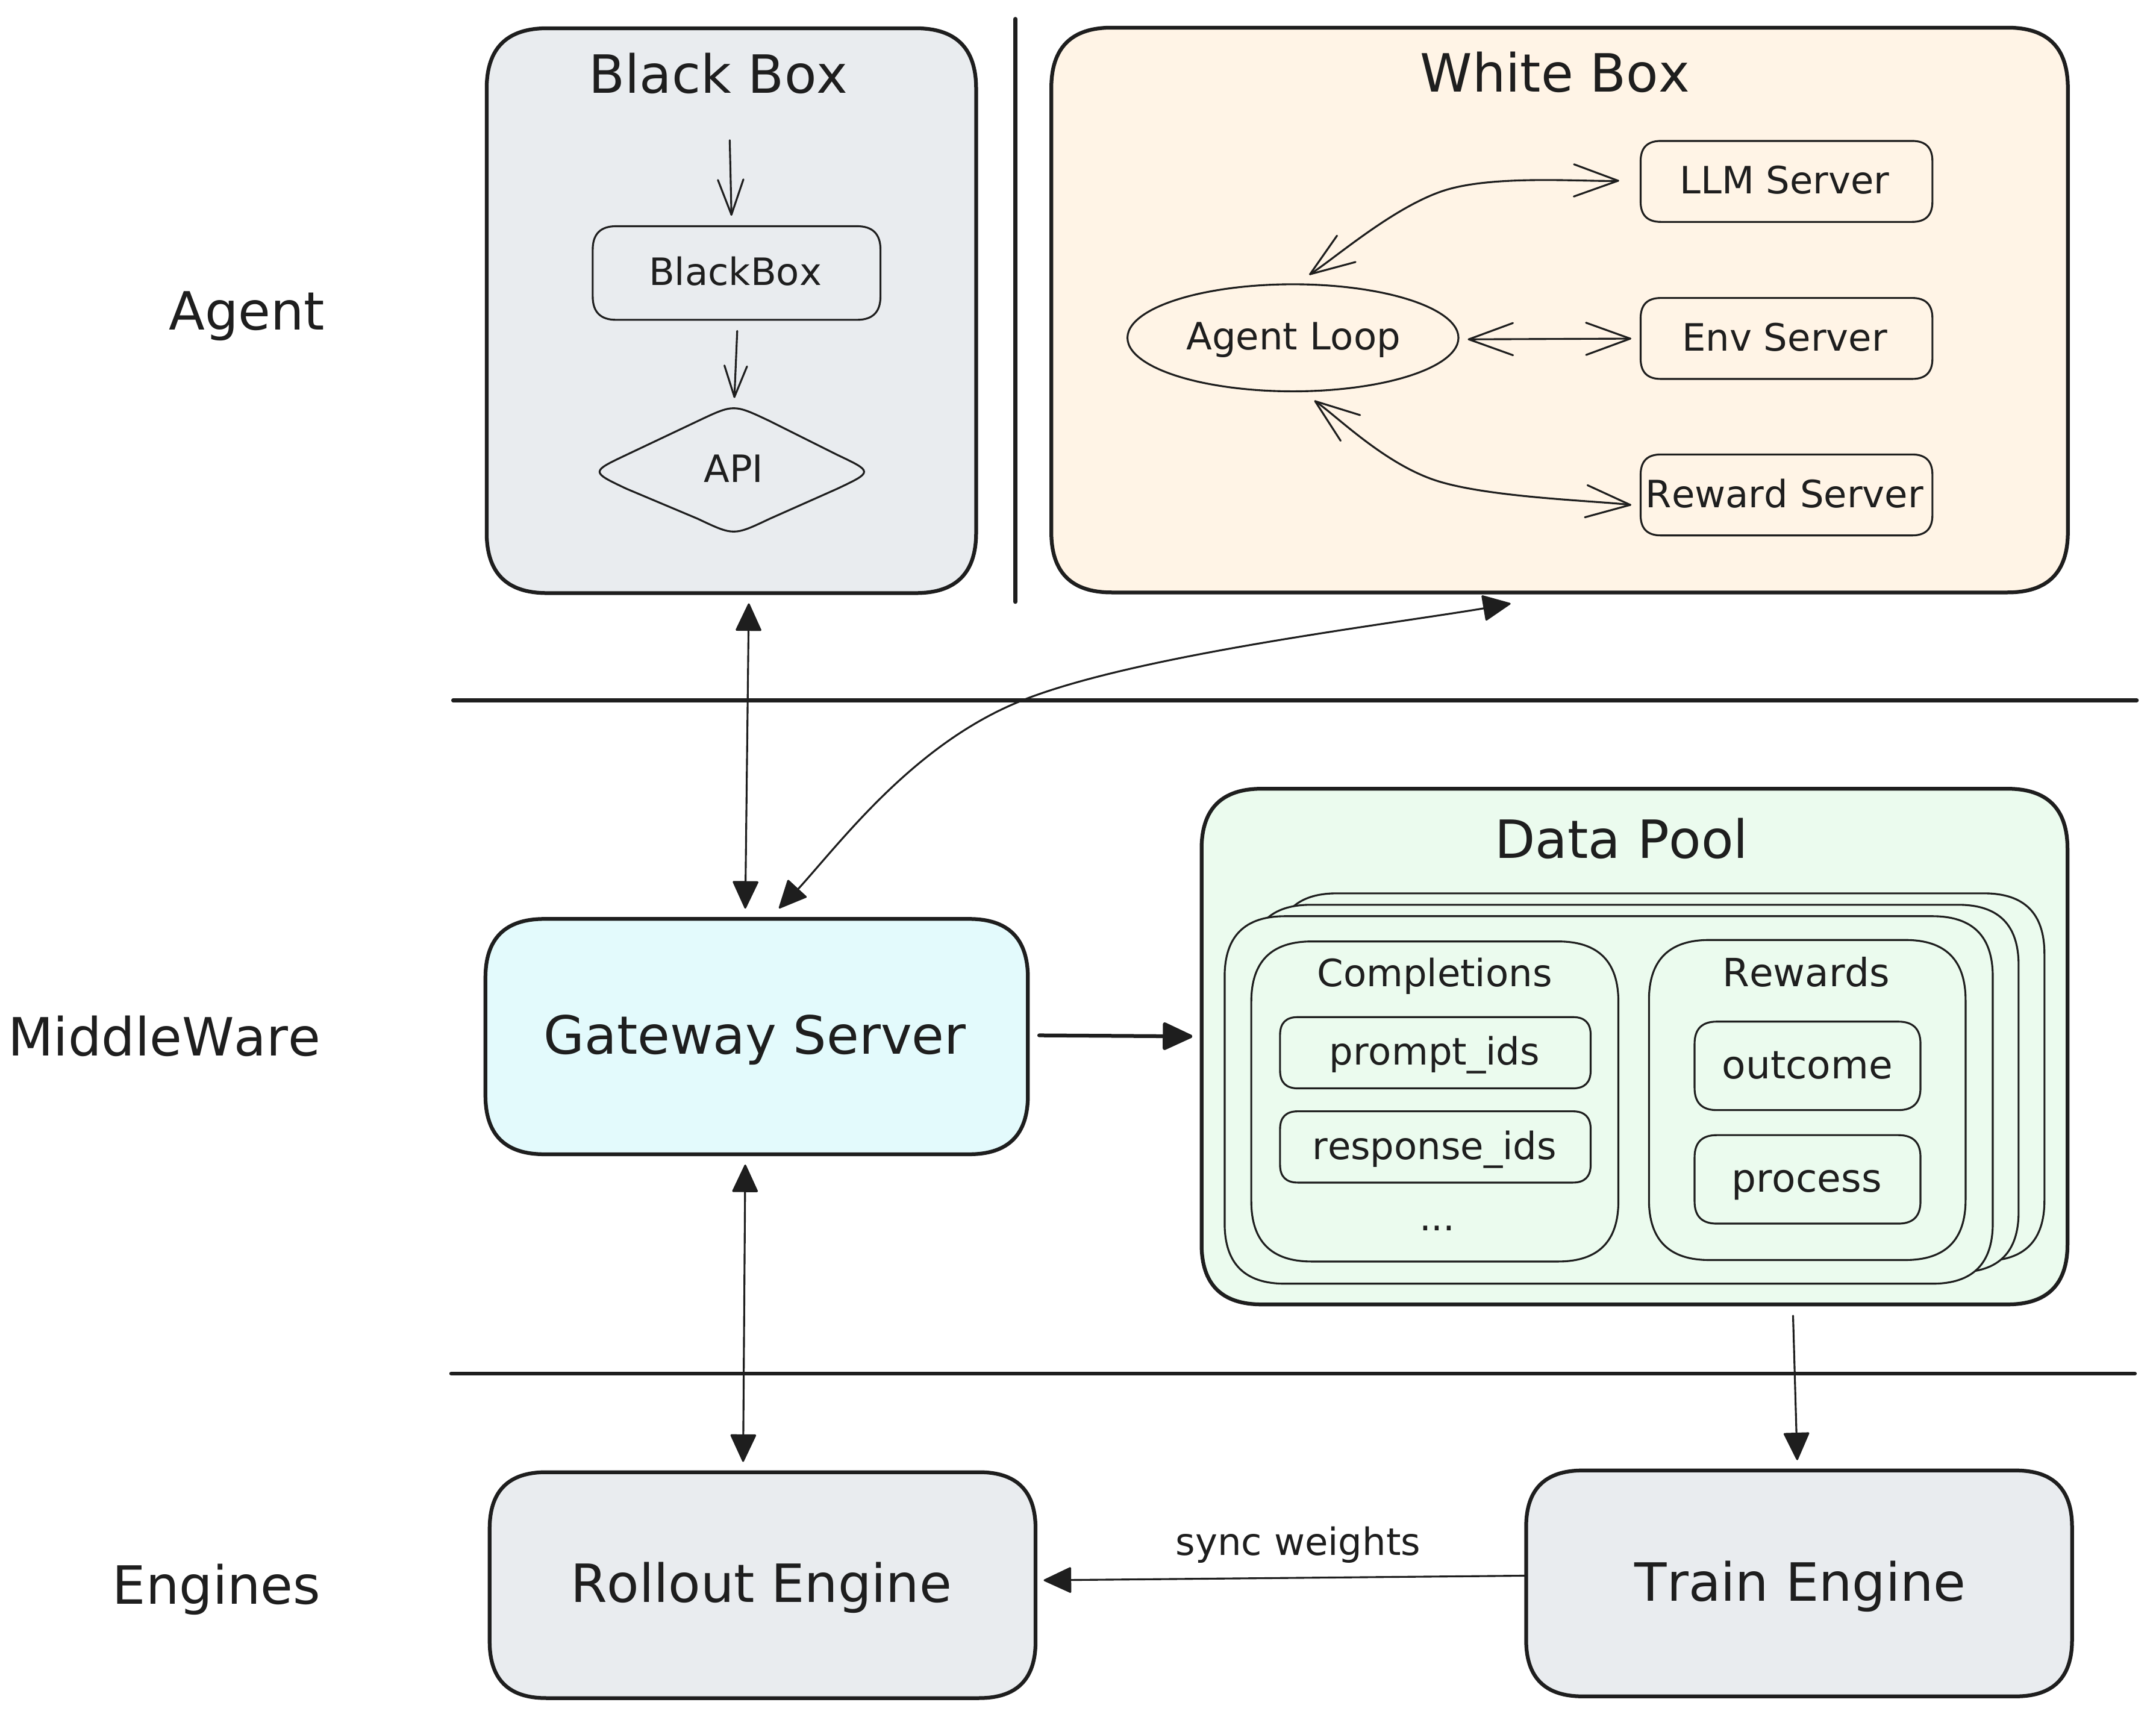
\includegraphics[width=0.78\textwidth]{figures_new/forge.pdf}
\caption{Overview of the Forge RL system. Three decoupled modules---Agent Side, Training/Inference Side, and the middleware abstraction layer (Gateway Server, Data Pool)---communicate through standardized interfaces, allowing the agent and the training loop to scale independently.}
\label{fig:forge-arch}
\end{figure}

\noindent \textbf{Agent Side.} This module encapsulates arbitrary agent implementations and orchestrates their interactions with external environments. Functioning as a pure trajectory producer, the agent side is entirely agnostic to training and inference mechanics. It drives the environment dynamics defined in the MDP formulation---executing tool calls, managing context, and accessing memory---and records the resulting $(s_t, a_t, o_t)$ tuples for downstream training consumption.

\noindent \textbf{Middleware Abstraction Layer.} Two components bridge the agent and training sides. The Gateway Server provides a standardized communication interface that routes completion requests between agents and the LLM engine, abstracting away the heterogeneity of agent scaffolds. The Data Pool serves as distributed trajectory storage that asynchronously collects rollout data, fully decoupling the generation and training pipelines and enabling each to scale independently.

\noindent \textbf{Training and Inference Side.} The Rollout Engine handles high-throughput token generation, serving as the policy $\pi_\theta$ that responds to Gateway requests. The Train Engine consumes processed trajectory sequences from the Data Pool, computes the CISPO policy gradient, and synchronizes updated weights back to the Rollout Engine.

\subsubsection{White-Box and Black-Box Agent Support}

The MDP formulation in the preceding subsection defines context management, tool execution, and memory access as environment dynamics. The infrastructure must support two distinct paradigms for how agents implement these dynamics, which differ in the degree of visibility the framework has into the agent's internal state.

\noindent \textbf{White-Box Agents} expose their context management logic to the training framework. The state transition $s_{t+1} = f_{\text{CM}}(\mathrm{concat}(s_t, a_t, o_t))$ is implemented within the framework itself, enabling the training pipeline to directly observe and backpropagate through context transformation operations. This tight integration allows the framework to construct training sequences that faithfully reflect the CM-induced distribution, ensuring that the policy is optimized over the true inference-time state distribution. White-box integration is particularly effective for agents with well-defined CM strategies (e.g., sliding-window truncation, periodic summarization), where the framework can reconstruct exact training states.

\noindent \textbf{Black-Box Agents} treat the agent as an opaque trajectory producer. Agents route completion requests to the RL service Gateway without exposing their internal context management, memory compression, or multi-agent coordination logic. The framework collects only the externally visible $(s_t, a_t, o_t)$ tuples---where $s_t$ is the context as presented to the LLM at each completion request---and constructs training data from these observations. This non-intrusive paradigm supports arbitrary internal architectures, including deep thinking loops, aggressive context rewriting, and hierarchical multi-agent systems, delivering consistent improvements without requiring any agent-side modifications.

The Gateway-based abstraction unifies both paradigms: white-box agents differ only in that their CM operations are registered with the framework for training-time reconstruction, while black-box agents rely solely on the observed request stream. This design has been validated across hundreds of distinct agent scaffolds and thousands of tool invocation formats.

\subsubsection{Windowed FIFO Scheduling}

Agent rollout completion times exhibit extreme variance---from seconds for simple API calls to hours for complex reasoning chains---creating a fundamental tension between throughput and distributional consistency. Strict FIFO scheduling preserves the data distribution but suffers from straggler-induced head-of-line (HoL) blocking. Fully greedy scheduling (fetching whichever trajectory completes first) maximizes throughput but causes severe distribution shift: early training batches are dominated by short, easy tasks, while hard tasks cluster in later batches, leading to gradient oscillation and optimization instability.

We propose \textbf{Windowed FIFO} (Figure~\ref{fig:window-fifo}), a hybrid scheduling strategy that interpolates between these extremes. Given a generation queue $Q = [T_0, T_1, \ldots, T_{N-1}]$ with current head index $i$, the training scheduler may only fetch completed trajectories within a sliding window $[T_i, T_{i+W-1}]$, where $W$ is the window size (e.g., $W = 0.3N$). Within the window, the scheduler operates greedily---any completed trajectory may be fetched immediately, mitigating HoL blocking. Across window boundaries, strict ordering is enforced: trajectories beyond the window are blocked regardless of completion status, and the window advances only as head-of-window tasks are consumed.

This provides a tunable trade-off controlled by $W$: smaller values approach strict FIFO (maximum distributional consistency), while larger values approach greedy scheduling (maximum throughput). In practice, $W = 0.3N$ maintains near-FIFO distributional properties while substantially reducing cluster idle time.

\begin{figure}[h]
\centering
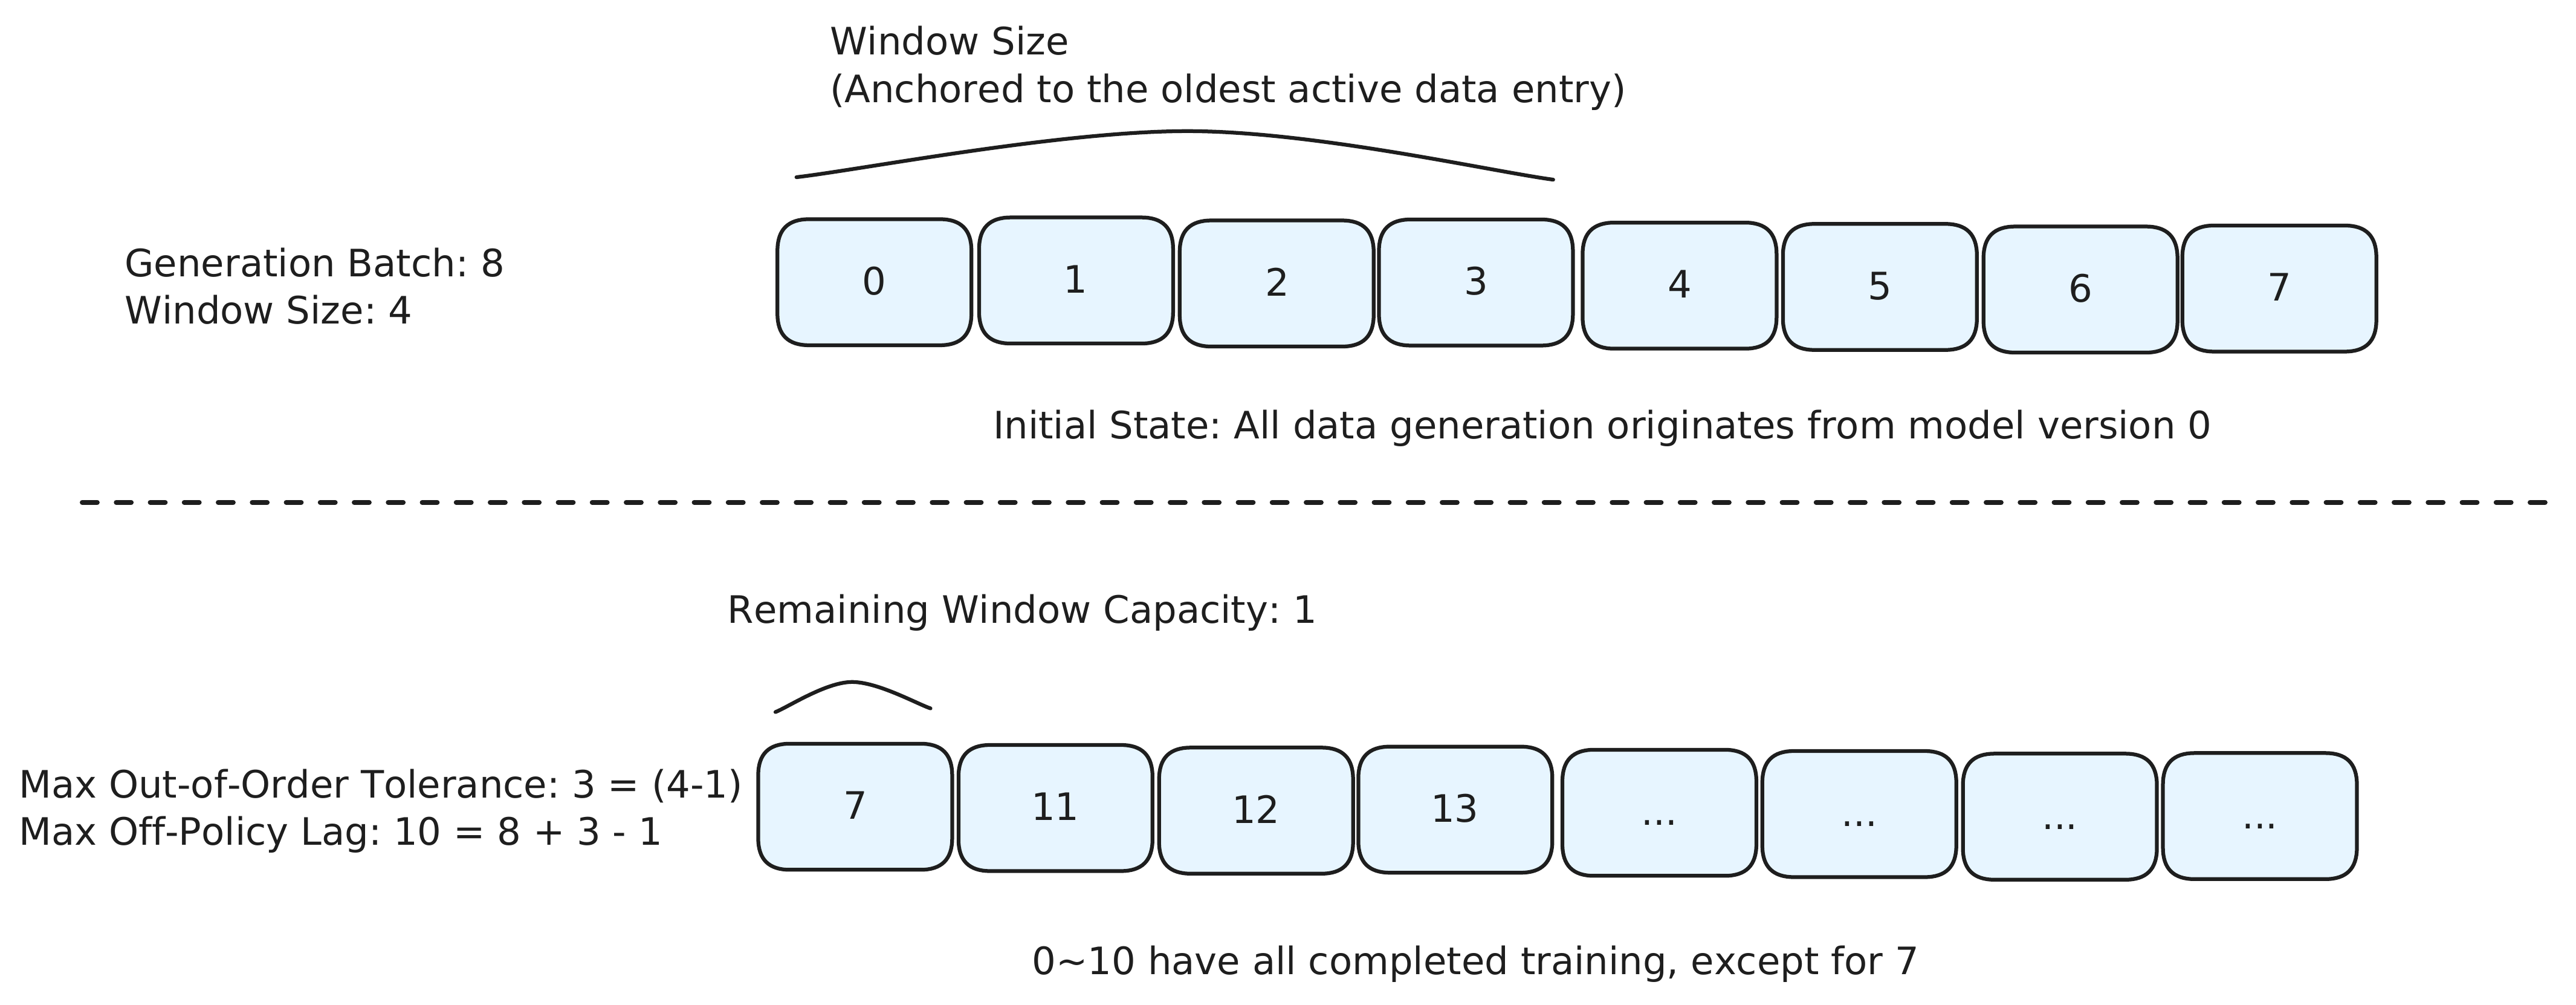
\includegraphics[width=0.95\textwidth]{figures_new/windowed_fifo.pdf}
\caption{Windowed FIFO scheduling. The training scheduler only fetches completed trajectories within a sliding window of size $W$ over the generation queue: within the window, completion order is free (mitigating head-of-line blocking); across window boundaries, strict FIFO is enforced (preserving distributional consistency).}
\label{fig:window-fifo}
\end{figure}

\subsubsection{Prefix Tree Merging for Training Acceleration}

In multi-turn agent trajectories, sequential message appending and context management operations produce extensive shared prefixes across training samples within the same rollout group. Traditional training treats each sample independently, redundantly recomputing common prefixes---a particularly severe source of waste in long-context agent scenarios.

We propose \textbf{prefix tree merging} (Figure~\ref{fig:prefix-tree-merge}), which restructures training computation from linear sample processing to tree-structured computation. Multiple completions sharing a common prefix are merged into a single prefix tree: the shared prefix is computed exactly once in the forward pass, after which the computation branches into individual response segments. After the forward pass, the tree is deconstructed using stored metadata, and loss is computed independently per sample.

This restructuring is mathematically equivalent to independent-sample training---the causal attention computation over a shared prefix produces identical activations regardless of whether it is computed once or $k$ times---guaranteeing zero approximation error. In practice, prefix tree merging achieves up to $40\times$ training speedup with corresponding reductions in memory consumption, enabling longer sequences and larger batch sizes without any compromise in training fidelity.

\begin{figure}[h]
\centering
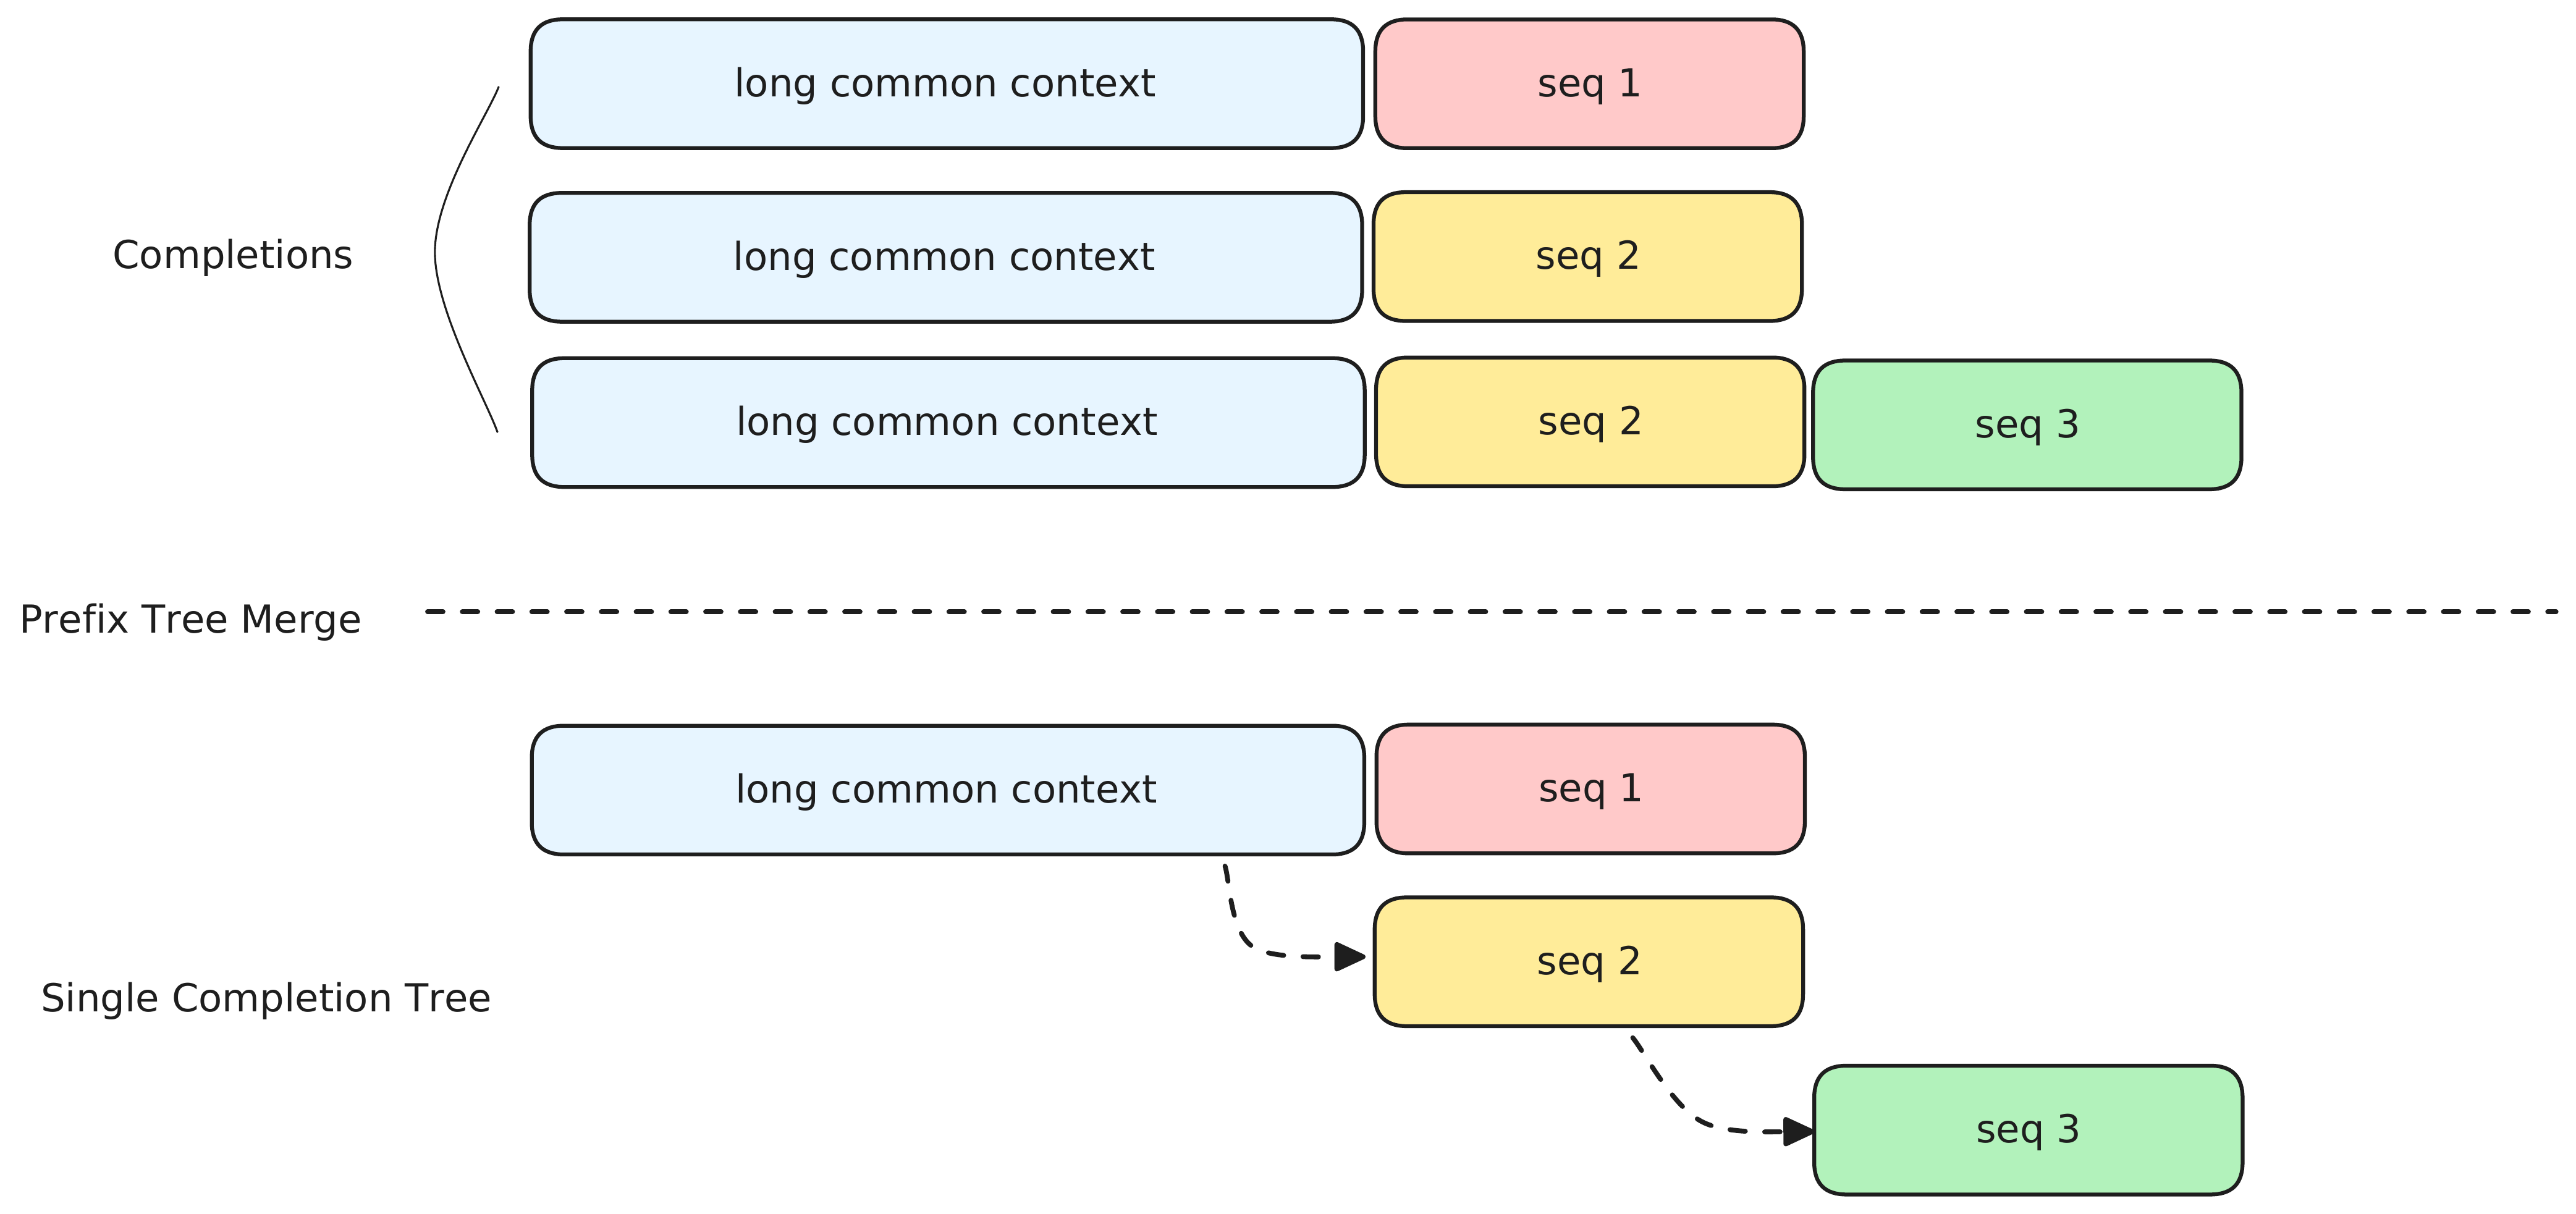
\includegraphics[width=0.95\textwidth]{figures_new/prefix_tree_merge.pdf}
\caption{Prefix tree merging. Completions that share a common prefix within a training batch are merged into a tree; the shared prefix is computed exactly once in the forward pass and the computation branches into individual response segments. The tree is deconstructed before the loss is computed independently per sample, so the procedure is mathematically equivalent to independent-sample training while eliminating redundant prefix recomputation.}
\label{fig:prefix-tree-merge}
\end{figure}

\subsubsection{Inference Acceleration}

We employ three architectural optimizations to maximize generation throughput for agent RL rollouts.

\noindent \textbf{MTP-based Speculative Decoding.} Multi-Token Prediction (MTP) modules are continuously co-trained with the RL policy via top-$K$ KL divergence loss. This co-training ensures that draft acceptance rates remain high throughout the non-stationary RL optimization process, preventing the distribution shift that would otherwise degrade speculative decoding performance as the policy evolves.

\noindent \textbf{Heterogeneous Prefill-Decode Disaggregation.} Prefill and decode operations are decoupled into independently scheduled instances, eliminating the mutual interference that arises from mixed scheduling in Mixture-of-Experts (MoE) architectures. Each phase adopts parallelism strategies optimized for its computational profile, simultaneously maximizing global throughput and minimizing tail latency.

\noindent \textbf{Global L3 KV Cache Pool.} A distributed, DFS-backed global KV cache maximizes prefix cache hit rates through group-level rollout scheduling. A cost-aware request router dynamically balances queuing delay against cache migration costs, maximizing cache locality without overloading individual instances and avoiding redundant prefilling across the multi-turn interactions characteristic of agent RL.
